% !TeX spellcheck = de_DE
\documentclass[12pt]{article}
\usepackage[utf8]{inputenc}
\usepackage{geometry}
\usepackage{svg}
\usepackage{float}
\usepackage{caption}
\usepackage{amsmath,amsthm,amsfonts,amssymb,amscd}
\usepackage{fancyhdr}
\usepackage{titlesec}
\usepackage{hyperref}
\usepackage{listings}
\usepackage[skip=3pt]{parskip}
\usepackage[ngerman]{babel}
\pagestyle{empty}
\titleformat*{\section}{\large\bfseries}
\titleformat*{\subsection}{\bfseries}

%
\geometry{
	a4paper,
	total={170mm,240mm},
	left=20mm,
	top=30mm,
}

\date{}
%Bitte ausfüllen
\newcommand\course{Betriebssysteme}
\newcommand\hwnumber{\large Portfolio 2}
\newcommand\Name{Fabian Sponholz}
\newcommand\Neptun{1561546}

%Matheinheiten
\newcommand\m{\:\textrm{m}}
\newcommand\M{\:\Big[\textrm{m}\Big]}
\newcommand\mm{\:\textrm{mm}}
\newcommand\MM{\:\Big[\textrm{mm}\Big]}
\newcommand\un{\underline}
\newcommand\s{\:\textrm{s}}
\newcommand\bS{\:\Big[\textrm{S}\Big]}
\newcommand\ms{\:\frac{\textrm{m}}{\textrm{s}}}
\newcommand\MS{\:\Big[\frac{\textrm{m}}{\textrm{s}}\Big]}
\newcommand\mss{\:\frac{\textrm{m}}{\textrm{s}^2}}
\newcommand\MSS{\:\Big[\frac{\textrm{m}}{\textrm{s}^2}\Big]}

%Trennlinie
\newcommand\separator{\rule{\linewidth}{0.5pt}}

%Bitte nicht einstellen
\renewcommand{\figurename}{Abbildung}
\renewcommand{\tablename}{Tabelle}
\pagestyle{fancyplain}
\headheight 35pt
\lhead{\Name\\\Neptun}
\chead{\textbf{ \hwnumber}}
\rhead{\course \\ \today}
\lfoot{}
\cfoot{}
\rfoot{\small\thepage}
\headsep 1.5em

\lstset{
	basicstyle=\ttfamily\small,
	columns=fullflexible,
	frame=single,
	frameround=tttt,
	rulecolor=\color{gray},
}
% http://www.bollchen.de/blog/2011/04/good-looking-line-breaks-with-the-listings-package/
\lstset{
	prebreak=\raisebox{0ex}[0ex][0ex]{\ensuremath{\hookleftarrow}},
	postbreak=\raisebox{0ex}[0ex][0ex]{\ensuremath{\hookrightarrow\space}},
	breaklines=true,
	breakatwhitespace=true,
	numbers=left,
	numberstyle=\scriptsize,
}
\lstset{
	backgroundcolor=\color{white},
	extendedchars=true,
	basicstyle=\footnotesize\ttfamily,
	showstringspaces=false,
	showspaces=false,
	numbers=left,
	numberstyle=\footnotesize,
	numbersep=9pt,
	tabsize=2,
	breaklines=true,
	showtabs=false,
	captionpos=b
}
\lstset{
	keywordstyle=\color{blue}\bfseries,
	ndkeywordstyle=\color{darkgray}\bfseries,
	identifierstyle=\color{black},
	commentstyle=\color{purple}\ttfamily,
	stringstyle=\color{red}\ttfamily
}

\begin{document}
	
\section*{Umgebung der Experimente}
Folgende Tabellen beschreiben das System, auf dem die Tests durchgeführt wurden.
\subsection*{Hardware-Spezifikation}
\begin{table}[h]
	\centering
	\begin{tabular}{|l|l|}
		\hline
		\textbf{Merkmal} & \textbf{Spezifikation} \\
		\hline
		CPU-Bezeichnung & AMD Ryzen 5 4500U with Radeon Graphics\\
		CPU-Architektur & x86 (AMD Renoir) \\
		CPU-Fertigungsverfahren & 7 nm (TSMC) \\
		\hline
		Anzahl Kerne / Threads & 6 / 6 \\
		Basistaktfrequenz & 2.3 GHz \\
		Maximale Boost-Taktfrequenz & 4.0 GHz \\
		\hline
		L1-Cache & 384 KB \\
		L2-Cache & 3 MB \\
		L3-Cache & 8 MB \\
		\hline
		TDP (Thermal Design Power) & 15 Watt \\
		Maximale Temperatur & 105 °C \\
		\hline
		Arbeitsspeicher & 8GB DDR4-3200 \\
		\hline
		Erscheinungsdatum & 07.01.2020 \\
		\hline
	\end{tabular}
\end{table}

\subsection*{Software-Umgebung}
\begin{table}[h]
	\centering
	\begin{tabular}{|l|l|}
		\hline
		\textbf{Merkmal} & \textbf{Spezifikation} \\
		\hline
		Betriebssystem & Arch Linux\\
		Kernel-Version & Linux 6.12.8-arch1-1\\
		\hline
		Java-Version & Java 21\\
		Java-Implementierung & java-21-openjdk\\
		\hline
	\end{tabular}
\end{table}

\section{Aufgabe 1 - Latenz bei Kommunikation mit Spinlock}
\subsection{Erste Ansätze zur Latenzmessung}
Bei der Kommunikation über Spinlocks wartet ein Thread auf die Freigabe einer Ressource, indem er fortwährend (z.B. in einer \texttt{while}-Schleife) überprüft, ob die Ressource frei ist. 
Um die Latenz zu messen, habe ich neben dem Main-Thread einen \texttt{Reader}-Thread erstellt, der auf die Freigabe einer Ressource (Boolean, der auf \texttt{true} gesetzt wird) wartet, und den Wert dann wieder auf \texttt{false} setzt. 
Nachdem der Main-Thread den Wert auf \texttt{true} gesetzt hat, wartet er wiederum, bis der Wert wieder auf \texttt{false} gesetzt wird.

Um Race Conditions beim Abfragen der Werte aus den While-Schleifen zu vermeiden, wird der Zugriff mithilfe von \texttt{synchronized} Setter- und Getter-Methoden geregelt.
Jeder Thread trägt immer, wenn er eine Nachricht vom anderen Thread erhält, einen Zeitstempel in Nanosekunden in eine ausreichend große Array-Liste ein, woraus später die Latenz berechnet wird.
Nun folgen Auszüge aus dem Source Code, die dies zeigen.

\begin{lstlisting}[language=java,caption={Spinlocks: Latenzmessung im Main Thread}]
for (int i = 0; i < recursions; i++) {
	// set lock to true -> send message
	setLock(true);;
	
	// wait for the return message
	while (getLock()) {
		// Do nothing (spinlock)
	}
	
	// add current time to list
	messageTimes.add(System.nanoTime());
}
\end{lstlisting}

\begin{lstlisting}[language=java,caption={Spinlocks: Latenzmessung im Reader Thread}]
while (!isInterrupted()) {
	while (!isInterrupted() && experiment.getLock() == false) {
		// do nothing (spinlock)
	}
	
	// Add the current time to the list
	experiment.getMessageTimes().add(System.nanoTime());
	
	if (isInterrupted()) break;
	
	// Reset the lock (main thread is waiting)
	experiment.setLock(false);
}
\end{lstlisting}


\subsection{Versuchsaufbau / Implementierung}
Im Ursprünglichen Versuchsaufbau habe ich für jeden Versuchsdurchlauf den \texttt{Reader}-Thread und das \texttt{Experiment}-Objekt neu erstellt und jeweils von jedem Experiment die minimale Latenz gespeichert.
Das Ergebnis des ersten Durchlaufs ist in Abbildung \ref{img:spinlock_first} dargestellt.

\begin{figure}[H]
	\centering
	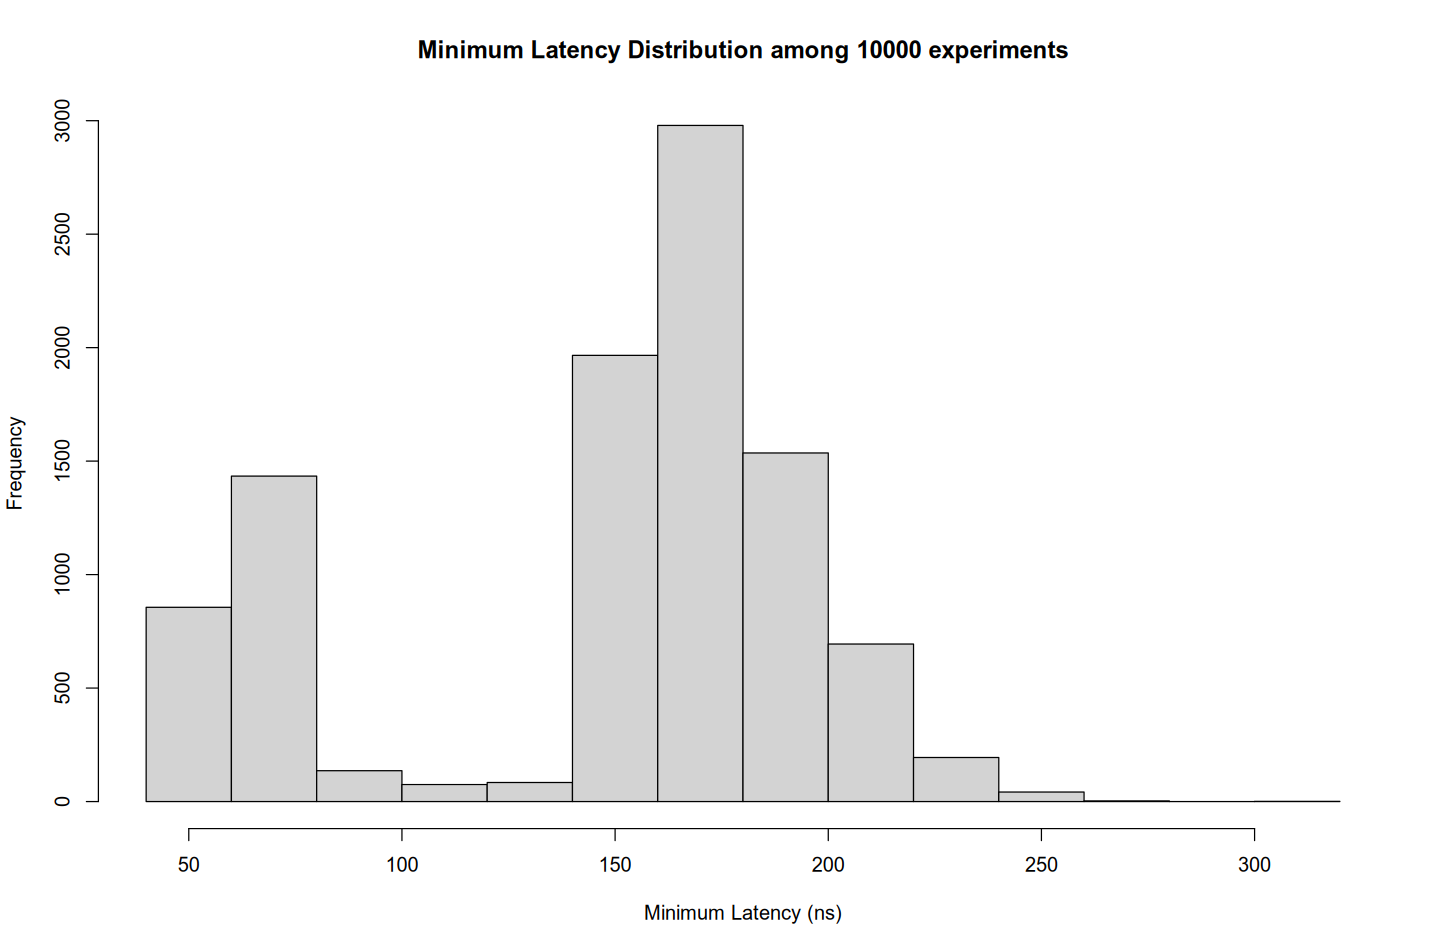
\includegraphics[width=0.75\textwidth]{./img/spinlock_first_try}
	\caption{Verteilung der Minima im ersten Experiment}
	\label{img:spinlock_first}
\end{figure}

Wie man sieht liegt, anders als zu erwarten wäre, keine Normalverteilung der Latenzen vor.
Nach reiflicher Überlegung hatte ich den Verdacht, dass ich durch die Instantiierung einer \texttt{Experiment}- und \texttt{Reader}-Objekts bei jedem Versuch eine große Menge ungenutzter Objekte erzeuge und dadurch ggf. der \emph{Garbage Collector} die Performance zeitweise mindert.

Um einen weiteren Performance-Faktor zu optimieren, habe ich noch die Konstruktion bestehend aus Boolean und synchronized Getter- und Settermethoden gegen einen \emph{AtomicBoolean} ausgetauscht.

Beim Herumexperimentieren wurde mir nun mit der Zeit klar, dass die Latenz derart gering sein muss, dass sie in der gleichen Größenordnung wie die Latenz der Zeitmessung selbst liegt.
Nachdem ich den Zeitmessungsprozess so weit ich konnte optimiert habe, sah der Prozess wie folgt aus:
\begin{lstlisting}[language=java,caption={Spinlocks: Latenzmessung im Main Thread (optimiert)}]
private void measure(int recursions) {
	long sendTime;
	long receiveTime;
	for (int i = 0; i < recursions; i++) {
		// Record time first, then
		sendTime = System.nanoTime();
		lock.set(true);
		while (lock.get()) {
			// Do nothing (spinlock)
		}
		receiveTime = System.nanoTime();
		
		sendTimes.add(sendTime);
		receiveTimes.add(receiveTime);
	}
}
\end{lstlisting}

\begin{lstlisting}[language=java,caption={Spinlocks: Reader Thread (optimiert)}]
while (!isInterrupted()) {
	while (!experiment.lock.get()) {
		// do nothing (spinlock)
	}
	
	// Reset the lock (main thread is waiting)
	experiment.lock.set(false);
}
\end{lstlisting}

So wird jeweils die Zeit für einen Turn-Around gemessen, also die Zeit, die die Information von Main-Thread zum Reader-Thread und wieder zurück braucht.
Zum Berechnen der Latenz wird diese Zahl später durch zwei geteilt.
Allerdings ist hier immer noch auch die Latenz für das Abfragen und Speichern der aktuellen Zeit enthalten, was das Ergebnis in einer solch niedrigen Größenordnung durchaus verfälschen kann.

\subsection{Ergebnis}
Schlussendlich habe ich mich mit dem Versuch so zufrieden gegeben.
Ich habe 10000 Durchläufe des Experiments mit jeweils 50000 Rekursionen durchgeführt und jeweils die Minimalwerte der einzelnen Experimente zusammengetragen.
Von 10000 Durchläufen betrug die minimale Latenz 9854 mal \textbf{genau 64 Nanosekunden}.
Das spricht dafür, dass wir hier bereits an die Grenzen der Messgenauigkeit stoßen und daher ist die Berechnung eines Konfidenzintervalls eigentlich hinfällig. Hier aber trotzdem die geforderten Werte, auch wenn \textbf{ihre Aussagekraft durchaus angezweifelt werden kann}:
\begin{itemize}
	\item Durchschnittliche Minimallatenz: $63,95 ns$
	\item Untere Schranke des 95\%-Konfidenzintervalls: $63,92 ns$
	\item Obere Schranke des 95\%-Konfidenzintervalls: $63,98 ns$
\end{itemize}

Hier noch eine Wertetabelle, die alle gemessenen Minimallatenzen aufzeigt.

\begin{table}[H]
	\centering
	\label{tab:latencies}
	\begin{tabular}{|r|r|}
		\hline
		Latenz ($ns$) & Häufigkeit \\
		\hline
		24 & 7 \\
		30 & 1 \\
		35 & 1 \\
		40 & 12 \\
		64 & 9854 \\
		65 & 124 \\
		120 & 1 \\
		\hline
	\end{tabular}
\end{table}

\section{Aufgabe 2 - Latenz bei Kommunikation durch Semaphore}
\subsection{Versuchsaufbau / Implementierung}

Da ich nun schon sehr viel Zeit mit der Optimierung der Messung in Aufgabe 1 verbracht habe, habe ich mich entschieden, die Lösung zur besseren Vergleichbarkeit nur leicht abzuwandeln und Semaphoren anstelle des \texttt{AtomicBoolean} und \texttt{while}-Schleifen zu verwenden.
Der Ansatz zur Zeitmessung bleibt hier der gleiche: 
Es gibt zwei Semaphoren, eine \texttt{messageSemaphore} und eine \texttt{replySemaphore}, die beide zunächst blockiert sind.
Der Reader-Thread versucht, sobald er läuft, den Lock auf der \texttt{messageSemaphore} zu bekommen und gibt, wenn er den Lock bekommen hat, die \texttt{replySemaphore} frei.
Die Zeitmessung läuft im Main-Thread nun wiefolgt ab:
\begin{enumerate}
	\item Beginn der Zeitmessung
	\item \texttt{messageSemaphore} freigeben
	\item Versuche, Lock auf \texttt{replySemaphore} zu erhalten (warte auf Reader-Thread)
	\item Wenn der Lock erfolgreich erhalten wurde, stoppe die Zeitmessung
\end{enumerate}

Hier ein Auszug der entsprechenden Stellen aus dem Code:

\begin{lstlisting}[language=java,caption={Semaphores: Latenzmessung im Main Thread}]
	private void measure(int recursions) {
		long sendTime;
		long receiveTime;
		for (int i = 0; i < recursions; i++) {
			// Record time first, then
			sendTime = System.nanoTime();
			messageSemaphore.release();
			replySemaphore.acquire();
			receiveTime = System.nanoTime();
			
			sendTimes.add(sendTime);
			receiveTimes.add(receiveTime);
		}
	}
\end{lstlisting}

\begin{lstlisting}[language=java,caption={Freigeben der replySemaphore im Reader Thread}]
	while (!isInterrupted()) {
		try {
			experiment.messageSemaphore.acquire();
			experiment.replySemaphore.release();
		} catch (InterruptedException e) {
			System.out.println("Reader Thread shutting down.");
			break;
		}
	}
\end{lstlisting}

So wird am ende durch Halbierung der gemessenen Zeit die durchschnittliche Latenz der beiden Wege berechnet und schließlich nach einer gegebenen Anzahl von Wiederholungen das Minimum abgespeichert.

\subsection{Ergebnis}
Bereits beim Testen ist mir anhand der Laufzeit aufgefallen, dass die Latenz bedeutend höher sein muss als in Aufgabe 1.
Um die Laufzeit gering zu halten, habe ich daher in dieser Versuchsreihe die Anzahl der Rekursionen auf 10000 reduziert und wie in Aufgabe 1 10000 Wiederholungen des Experiments durchgeführt.
Hier die Verteilung der Minimalen Latenzen über die 10000 Experimente:

\begin{figure}[H]
	\centering
	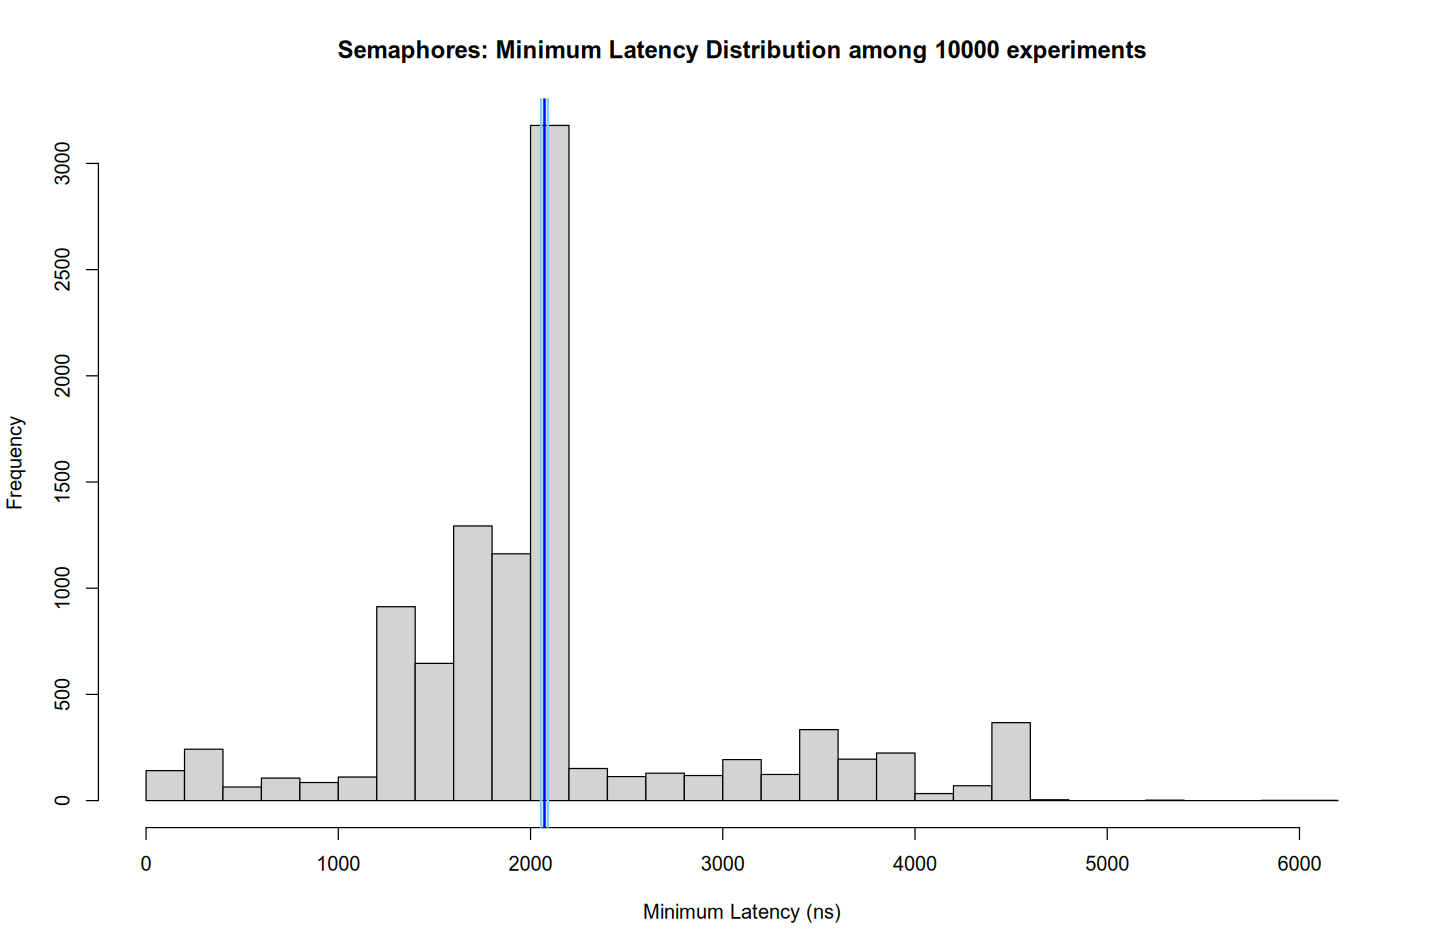
\includegraphics[width=0.75\textwidth]{./img/semaphores}
	\caption{Verteilung der Minima in der Versuchsreihe zu Aufgabe 2}
	\label{img:semaphore}
\end{figure}

Auch wenn sich hier eine Linksschiefe der Verteilung bemerkbar macht, gehe ich bei der Berechnung des Konfidenzintervalls (in Blau dargestellt) von einer Normalverteilung aus.
Der Grund für die Linksschiefe des Ergebnisses ist mir nicht ersichtlich.
Hier die Daten des 95\%-Konfidenzintervalls:
\begin{itemize}
	\item Durchschnittliche Minimallatenz: $2073 ns$
	\item Untere Schranke des 95\%-Konfidenzintervalls: $2055 ns$
	\item Obere Schranke des 95\%-Konfidenzintervalls: $2090 ns$
\end{itemize}

Die Latenz ist also um etwa zwei Zehnerpotenzen höher als bei der Verwendung von Spinlocks.
Dies ist auch nur logisch, da ein Thread in einem Spinlock alle ihm zur Verfügung stehenden Ressourcen verwendet, um zu überprüfen, ob der Lock freigegeben wurde.
Somit wird damit eine nahezu perfekte Latenz erzielt, jedoch bezahlt man den Preis dafür mit der CPU-Last, die ein Spinlock im Vergleich zu einer Semaphore hervorruft.
Wird ein Thread durch eine Semaphore blockiert, so wird er schlafen gelegt und verursacht nur eine sehr niedrige CPU-Last.

\end{document}